\chapter{Deep Learning}
\thispagestyle{fancy}
\label{chap:Deep Learning}
\noindent
Deep Learning ist ein Teilbereich des \ac{ML}. \ac{ML}-Algorithmen analysieren Daten automatisiert mittels mathematischer Methoden der Mustererkennung. \ac{DL}-Algorithmen bedienen sich hingegen vielschichtiger und hoch parametrisierter neuronaler Netze, um dem menschlichen Gehirn bestmöglich nachzuempfinden \cite[S.~455-457]{KHA19}. Dabei werden sehr große Datenmengen verarbeitet und analysiert, um einen Lerneffekt zu erzielen. Neben einer Eingabe- und einer Ausgabeschicht sorgen insbesondere die verborgenen Schichten für die prädizierte Tiefe. Hier werden Informationen weiterverarbeitet, abstrahiert und reduziert \cite[S.~131]{ZHA20}. Die potenziellen Einsatzmöglichkeiten gehen über die der \ac{ML}-Algorithmen hinaus. Der Aufbau neuronaler Netze sowie deren Funktionsweise und ausgewählte Architekturen werden in diesen Kapitel thematisiert. Hyperparameter und \ac{TL} schließen sich an.


\section{Neuronale Netze}
\noindent
Um den Aufbau und die Funktionsweise neuronaler Netze verstehen zu können, bedarf es zunächst der Beschreibung von Neuronen. Diese können im biologischen Sinne als Schalter verstanden werden, welche verschiedene Signale empfangen können und aktiviert werden, sobald genug Signale registriert wurden. Diese Aktivierung sendet folglich weitere Signale an andere Neuronen, wie \autoref{pic:ArtificialNeuron} im technischen Sinne exemplarisch skizziert \cite[S.~42]{KRI05}. Hierfür werden Aktivierungsfunktionen benötigt, welche die gewichteten Eingangssignale in ein Ausgangssignal konvertieren. Sie ermöglichen es, nicht-lineare Zusammenhänge zwischen den Eingangs- und den Ausgangsdaten herzustellen \cite[S.~134]{ZHA20}.\\

\begin{figure}[h!]
  \centering
  \fbox{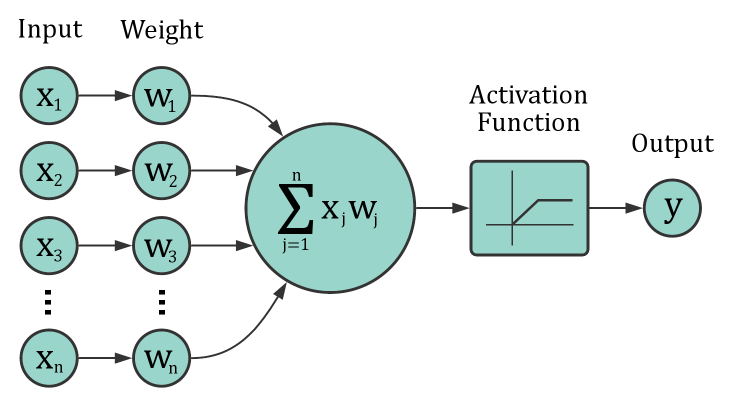
\includegraphics[width=0.6\linewidth]{./source/images/artificialneuron.png}}
  \caption{Aufbau eines künstlichen Neurons \cite{MCC20}.}
  \label{pic:ArtificialNeuron}
\end{figure}

\noindent
Die elementarste Form neuronaler Netze wird \ac{MLP} genannt. \ac{MLP} bestehen aus mehreren Schichten, deren Neuronen jeweils vollständig mit den Neuronen der umliegenden Schichten verbunden sind \cite[S.~131]{ZHA20}. Der Verständlichkeit halber veranschaulicht \autoref{pic:MultiLayerPerceptron} einen solchen Aufbau mit nur einer verborgenen Schicht, welche aus fünf Neuronen besteht.

\begin{figure}[h!]
  \centering
  \fbox{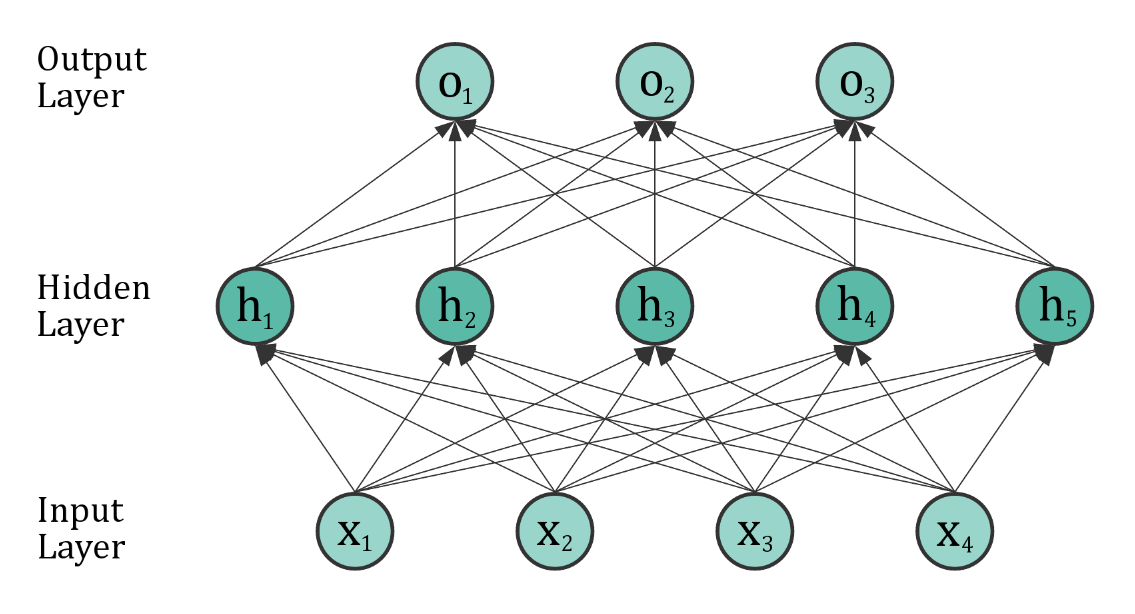
\includegraphics[width=0.6\linewidth]{./source/images/multilayerperceptron.png}}
  \caption{Aufbau eines MLP \cite[S.~133]{ZHA20}.}
  \label{pic:MultiLayerPerceptron}
\end{figure}

\noindent
Ziel der hoch parametrisierten neuronalen Netze ist es, komplexe Funktionen hohen Grades bestmöglich zu approximieren und so verschiedenste Probleme zu lösen. Der anvisierte Lerneffekt wird mithilfe des sogenannten Backpropagation-Algorithmus erreicht. Hierbei werden Eingangsdaten zunächst vorwärts durch ein neuronales Netz hindurch propagiert. Mithilfe einer Fehlerfunktion wird sodann die erwartete mit der tatsächlichen Ausgabe verglichen und bewertet. Über das Gradientenverfahren werden die Fehler nun rückwärts durch das neuronale Netz propagiert und somit die Gewichte in den Neuronen angepasst, insbesondere in den verborgenen Schichten. Ziel ist die Minimierung der Fehlerfunktion und letztlich die Optimierung der durch das neuronale Netz approximierten Funktion \cite[S.~140, 169]{ZHA20}.\\

\noindent
Der Trainingsprozess erfolgt optimalerweise über mehrere sogenannte Epochen. Hier werden dem neuronalen Netz verschiedene Eingangsdaten zugeführt und beidseitige Propagationen ausgeführt. Wichtig ist dennoch, kein Overfitting beziehungsweise Underfitting zu erzeugen. Dies würde bedeuten, dass das trainierte Modell zu sehr beziehungsweise zu wenig auf die Trainingsdaten angepasst ist. Ziel ist ein möglichst hoher Generalisierungseffekt des Modells, wie \autoref{pic:FittingTypes} zeigt. Das Modell sollte den Lernfortschritt auf noch unbekannte Daten adaptieren können und darauf eine hohe Genauigkeit erreichen. Es gibt verschiedene Ansätze, um beispielsweise Overfitting vorzubeugen. Hier seien insbesondere Batch Normalization und Dropout genannt, wobei entsprechende Mechanismen an anderweitiger Stelle erläutert werden \cite[S.~143-149]{ZHA20}.

\begin{figure}[h!]
  \centering
  \fbox{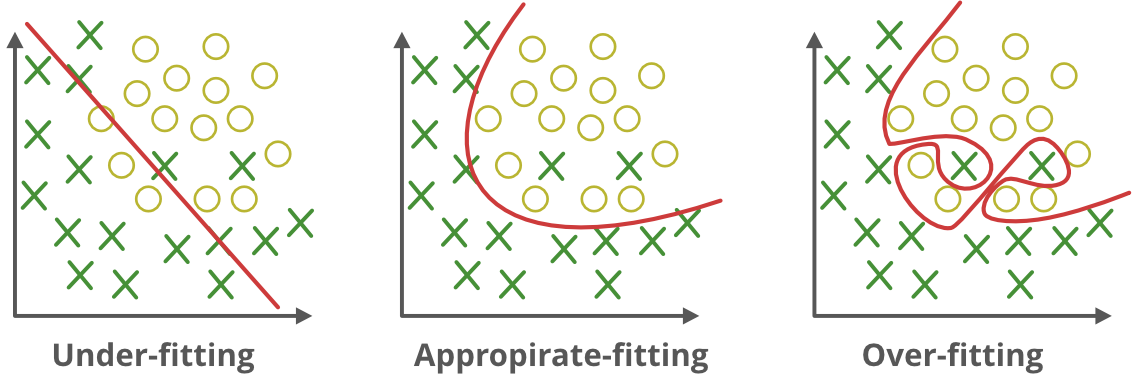
\includegraphics[width=0.6\linewidth]{./source/images/fittingtypes.png}}
  \caption{Typen von Generalisierungseffekten \cite{EDPOJ}.}
  \label{pic:FittingTypes}
\end{figure}


\section{Architekturen}
\noindent
Um mithilfe neuronaler Netze die \ac{ATS} zu modellieren, werden nun ausgewählte Architekturen vorgestellt. Diese gehen weit über die als Grundlage beschriebenen \ac{MLP} hinaus und verdeutlichen die Varietät neuronaler Netze. 


\subsection{Recurrent Neural Networks}
\cite{ZHA20} ab Seite 361, 354


\subsection{Encoder-Decoder Networks}
\cite{ZHA20} ab Seite 377, 375, YAN19 S. 3 links unten, S. 3 rechts unten


\subsection{Attention in Neural Networks}
\cite{ZHA20} ab Seite 389, 394 mit Self-Attention, Multi-Head-Attention


\subsection{Transformer Networks}
\cite{ZHA20} ab Seite 398 mit MH-Attention, Encoder, Decoder, Training etc.


\section{Hyperparameter}
\noindent
Hyperparameter sind Parameter einer Architektur, die bereits vor dem eigentlichen Trainingsprozess definiert werden. Sie sind dennoch optimierbar und beeinflussen den Trainingsfortschritt enorm. Als Hyperparameter gelten insbesondere die Learning Rate, die Anzahl der Epochen oder auch das Momentum. Eine sogenannte Grid Search ist in der Lage, die Hyperparameter automatisiert zu optimieren, bedarf aber dennoch einer gewissen Zeit.

Notizen:
\begin{itemize}
	\item \cite{ZHA20} ab Seite 413 in den Unterkapiteln schauen
	\item Hyperparameter vorstellen, bspw. siehe Website + Quellen
	\item Notwendigkeit und Einfluss von Hyperparametern beschreiben
	\item Batch-Size, e.g. Mini-Batch vs. Stochastic Batch: \url{https://stats.stackexchange.com/questions/153531/what-is-batch-size-in-neural-network}
\end{itemize}


\section{Transfer Learning}
\noindent
\ac{TL} ist in den letzten Jahren wissenschaftlich immer bedeutsamer geworden, da \ac{DL}-Modelle heutzutage sehr komplex und Trainingsprozesse sehr zeit- und rechenintensiv sind. Unter \ac{TL} versteht man das Wiederverwenden bereits vortrainierter neuronaler Netze für die Lösung neuartiger Probleme. Dabei werden die erprobten Modelle als Startpunkt genutzt und nur noch auf die neuen Probleme adaptiert, anstatt eigene Modelle von Grund auf neu zu trainieren. Anwender profitieren hier zeitlich, qualitativ und technisch. Zumeist sind architektonische Anpassungen in den hinteren Schichten der vortrainierten Modelle erforderlich, sodass sie sich für die Lösung der neuen Probleme eignen, wie \autoref{pic:FineTuning} veranschaulicht. Zudem ist ein gezieltes weitergehendes Training mit entsprechenden Daten notwendig. Inwieweit die neuen Daten auf die vortrainierten Modelle einwirken sollen, ist individuell zu erproben \cite[S.~554]{ZHA20}.

\begin{figure}[h]
  \centering
  \fbox{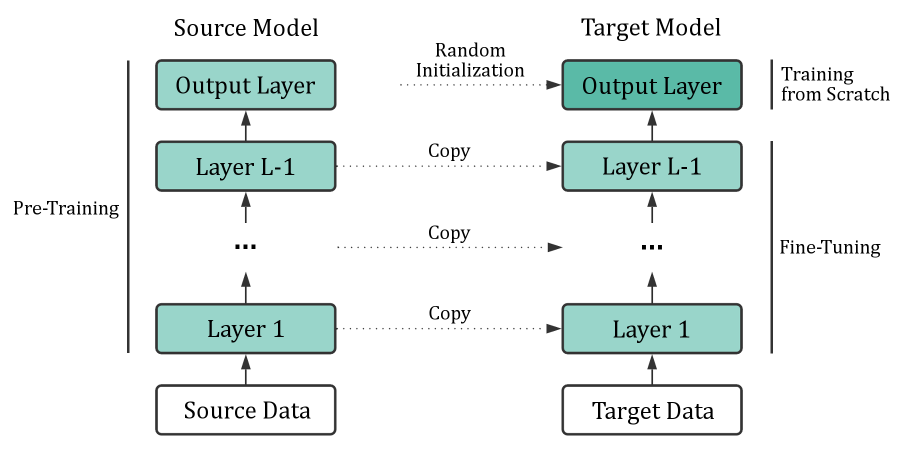
\includegraphics[width=0.6\linewidth]{./source/images/finetuning.png}}
  \caption{Fine-Tuning vortrainierter Modelle \cite[S.~555]{ZHA20}.}
  \label{pic:FineTuning}
\end{figure}

\noindent
\ac{TL} wird auch in dieser Arbeit genutzt. Einige Komponenten der bereits vorgestellten Architekturen, wie beispielsweise der Encoder oder auch der Decoder, können durch vortrainierte Modelle repräsentiert werden. Hier wird inhaltlich sowie kontextuell in den folgenden Kapiteln angeknüpft, da zunächst die Einführung weiterer \ac{NLP}-Grundlagen erforderlich ist. Die angeführten Vorteile von \ac{TL} können nichtsdestotrotz wie folgt zusammengefasst werden:

\begin{itemize}
	\item Zeitersparnis durch Überspringen des initialen Trainings
	\item Qualitätsanstieg und Generalisierung durch Berücksichtigung massenhafter Daten
	\item Reduktion der hardwaretechnischen Anforderungen und des Stromverbrauches
\end{itemize}
